\begin{ex}
 (Uff) Hoje em dia, é possível realizar diversas operações bancárias a partir de um computador pessoal ligado à internet. Para esse acesso, o cliente de determinado banco, após digitar o número de sua agência e conta corrente, deverá introduzir uma senha de 4 dígitos a partir de um teclado virtual como o da figura:

\begin{center}
\tikzset{every picture/.style={line width=0.75pt}} %set default line width to 0.75pt        

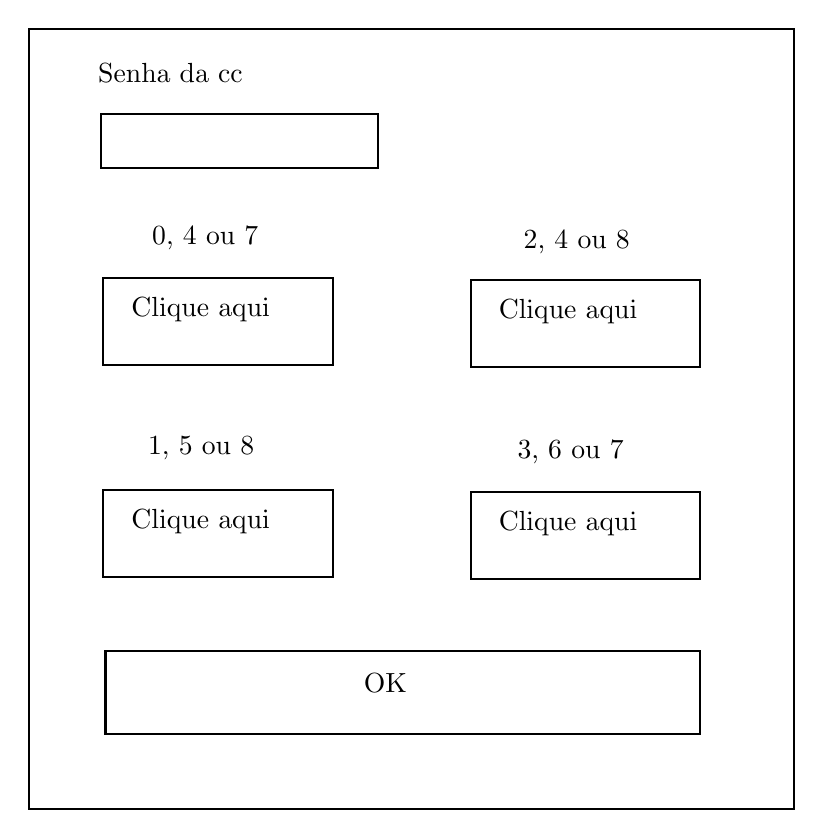
\begin{tikzpicture}[x=0.75pt,y=0.75pt,yscale=-1,xscale=1]
%uncomment if require: \path (0,409); %set diagram left start at 0, and has height of 409

%Shape: Rectangle [id:dp243297938897447] 
\draw   (146,23) -- (514.5,23) -- (514.5,399.13) -- (146,399.13) -- cycle ;
%Shape: Rectangle [id:dp04162812434187324] 
\draw   (181,64) -- (314.5,64) -- (314.5,90.13) -- (181,90.13) -- cycle ;
%Shape: Rectangle [id:dp7273870414239203] 
\draw   (182,143.13) -- (292.5,143.13) -- (292.5,185) -- (182,185) -- cycle ;
%Shape: Rectangle [id:dp8244344412524076] 
\draw   (183,323) -- (469.5,323) -- (469.5,363) -- (183,363) -- cycle ;
%Shape: Rectangle [id:dp5969374587945431] 
\draw   (359,144.13) -- (469.5,144.13) -- (469.5,186) -- (359,186) -- cycle ;
%Shape: Rectangle [id:dp9778166750565478] 
\draw   (182,245.13) -- (292.5,245.13) -- (292.5,287) -- (182,287) -- cycle ;
%Shape: Rectangle [id:dp4111016721980858] 
\draw   (359,246.13) -- (469.5,246.13) -- (469.5,288) -- (359,288) -- cycle ;

% Text Node
\draw (178,38) node [anchor=north west][inner sep=0.75pt]   [align=left] {Senha da cc};
% Text Node
\draw (194,151) node [anchor=north west][inner sep=0.75pt]   [align=left] {Clique aqui};
% Text Node
\draw (306,332) node [anchor=north west][inner sep=0.75pt]   [align=left] {OK};
% Text Node
\draw (371,152) node [anchor=north west][inner sep=0.75pt]   [align=left] {Clique aqui};
% Text Node
\draw (194,253) node [anchor=north west][inner sep=0.75pt]   [align=left] {Clique aqui};
% Text Node
\draw (371,254) node [anchor=north west][inner sep=0.75pt]   [align=left] {Clique aqui};
% Text Node
\draw (204,117) node [anchor=north west][inner sep=0.75pt]   [align=left] {0, 4 ou 7};
% Text Node
\draw (383,119) node [anchor=north west][inner sep=0.75pt]   [align=left] {2, 4 ou 8};
% Text Node
\draw (202,218) node [anchor=north west][inner sep=0.75pt]   [align=left] {1, 5 ou 8};
% Text Node
\draw (380,220) node [anchor=north west][inner sep=0.75pt]   [align=left] {3, 6 ou 7};


\end{tikzpicture}
\end{center}




Para inserir um dígito da senha de sua conta corrente, o cliente deste banco deve clicar em um dos 4 botões "clique aqui"; isto é, para inserir o dígito 4, por exemplo, pode-se clicar no botão "clique aqui" situado abaixo dos dígitos "0, 4 ou 7" ou naquele situado abaixo dos dígitos "2, 4 ou 8".

Pode-se afirmar que o número total de senhas compostas por 4 dígitos distintos que estão associados à sequência de "cliques", primeiro no botão correspondente aos dígitos 1, 5 ou 8; depois, no botão correspondente aos dígitos 0, 4 ou 7; novamente no botão correspondente aos dígitos 1, 5 ou 8 e, por último, no botão correspondente aos dígitos 0, 4 ou 7, é igual a:
    \begin{enumerate}[(a)]
    \item 12
    \item 24
    \item 36
    \item 54
    \item 81
    \end{enumerate}
      \begin{sol}
        resposta: c  \\
        ordem dos botões: $(1,5,8)\rightarrow(0,4,7)\rightarrow(1,5,8)\rightarrow(0,4,7)$ \\
        número de dígitos possíveis: $3\cdot3\cdot2\cdot2=36$
      \end{sol}
\end{ex}